% !TeX encoding = UTF-8
% !TeX program = xelatex

\documentclass[type=master]{sjtuthesis}
% !TEX root = ./main.tex

% 工作标题及个人信息。正式提交前核对学院规定并填写真实信息。
\sjtusetup{
  info = {%
    zh / title      = {面向关系表格学习的语义建模与高效训练方法研究},
    en / title      = {Semantic Modeling and Efficient Training Methods for Relational Table Learning},
    zh / keywords   = {关系表格学习, 元路径, 异构图, 按需训练},
    en / keywords   = {relational table learning, meta-path, heterogeneous graph, on-demand training},
    zh / author     = {待填写},
    en / author     = {To be completed},
    id              = {待填写},
    zh / supervisor = {待填写},
    en / supervisor = {To be completed},
    zh / department = {待填写},
    en / department = {To be completed},
    zh / major      = {待填写},
    en / major      = {To be completed},
    zh / degree     = {待填写},
    en / degree     = {To be completed},
    zh / display-date = {待填写},
  },
}

% 使用 BibLaTeX 处理参考文献
%   biblatex-gb7714-2015 常用选项
%     gbnamefmt=lowercase     姓名大小写由输入信息确定
%     gbpub=false             禁用出版信息缺失处理
\usepackage[backend=biber,style=gb7714-2015]{biblatex}
% 文献表字体
\renewcommand{\bibfont}{\zihao{5}\setbaselineskip{16bp}}
% 文献表条目间的间距
\setlength{\bibitemsep}{3bp plus 1pt}
% 导入参考文献数据库
\addbibresource{refs.bib}

% 脚注格式
\usepackage[perpage,bottom,hang]{footmisc}

% 定义图片文件目录与扩展名
\graphicspath{{figures/}}
\DeclareGraphicsExtensions{.pdf,.eps,.png,.jpg,.jpeg}

% 颜色宏包
\usepackage{xcolor} 

% 写作阶段的可见占位文字；定稿时逐段替换。
\newcommand{\thesisplaceholder}[1]{%
  \par\smallskip\noindent{\color{gray}\itshape 待补充：#1}\par\smallskip
}

% 确定浮动对象的位置，可以使用 [H]，强制将浮动对象放到这里（可能效果很差）
% \usepackage{float}

% 固定宽度的表格
% \usepackage{tabularx}

% 使用三线表：toprule，midrule，bottomrule。
\usepackage{booktabs}

% 表格中支持跨行
\usepackage{multirow}

% 表格中数字按小数点对齐
\usepackage{dcolumn}
\newcolumntype{d}[1]{D{.}{.}{#1}}

% 使用长表格
\usepackage{longtable}

% 附带脚注的表格
\usepackage{threeparttable}

% 附带脚注的长表格
\usepackage{threeparttablex}

% 算法环境宏包
\usepackage[ruled,vlined,linesnumbered]{algorithm2e}
% \usepackage{algorithm, algorithmicx, algpseudocode}

% 代码环境宏包
\usepackage{listings}
\lstdefinestyle{lstStyleCode}{%
  aboveskip         = \medskipamount,
  belowskip         = \medskipamount,
  basicstyle        = \ttfamily\zihao{-5}\setbaselineskip{12bp},
  commentstyle      = \slshape\color{black!60},
  stringstyle       = \color{green!40!black!100},
  keywordstyle      = \bfseries\color{blue!50!black},
  extendedchars     = false,
  upquote           = true,
  tabsize           = 2,
  showstringspaces  = false,
  xleftmargin       = 1em,
  xrightmargin      = 1em,
  breaklines        = false,
  framexleftmargin  = 1em,
  framexrightmargin = 1em,
  backgroundcolor   = \color{gray!10},
  columns           = flexible,
  keepspaces        = true,
  % texcl             = true,  % 代码中的注释部分将会被视为 LaTeX 正文模式内容
  % mathescape        = true,  % 代码中$..$的部分将会被视为 LaTeX 数学模式内容
}
\lstnewenvironment{codeblock}[1][]{%
  \lstset{style=lstStyleCode,#1}}{}

% 直立体数学符号
\providecommand{\dd}{\mathop{}\!\mathrm{d}}
\providecommand{\ee}{\mathrm{e}}
\providecommand{\ii}{\mathrm{i}}
\providecommand{\jj}{\mathrm{j}}

% 国际单位制宏包
\usepackage{siunitx}

% 定理环境宏包
\usepackage{amsthm}
% \usepackage{ntheorem}

% 绘图宏包
\usepackage{tikz}
\usetikzlibrary{arrows.meta, shapes.geometric}

% 数据图表宏包
\usepackage{pgfplots}
\pgfplotsset{compat=newest}

% 一些文档中用到的 logo
\usepackage{hologo}
\providecommand{\XeTeX}{\hologo{XeTeX}}
\providecommand{\BibLaTeX}{\textsc{Bib}\LaTeX}

% 借用 ltxdoc 里面的几个命令方便写文档
\DeclareRobustCommand\cs[1]{\texttt{\char`\\#1}}
\providecommand\pkg[1]{{\sffamily#1}}

% hyperref 宏包在最后调用
\usepackage{hyperref}

% E-mail
\providecommand{\email}[1]{\href{mailto:#1}{\urlstyle{tt}\nolinkurl{#1}}}


\begin{document}

\maketitle
\copyrightpage

\frontmatter
% !TEX root = ../main.tex

\begin{abstract}[zh]
  \thesisplaceholder{约 500 字概述关系表格学习的背景与问题、MetaRTL 的方法和结果、RelX 的设计和结果，并给出两项工作的结论。实验结果须与正文最终数据一致。}
\end{abstract}

\begin{abstract}[en]
  \noindent\textit{To be completed: Provide an English abstract corresponding to the final Chinese abstract, including the problem, methods, verified results, and conclusions for MetaRTL and RelX.}
\end{abstract}

\tableofcontents
% 待补充术语表、插图索引和表格索引时，再启用对应命令。

\mainmatter
% !TEX root = ../main.tex

\chapter{绪论}
\label{chap:introduction}

\section{研究背景与意义}

关系数据库是组织结构化数据的主要形式之一。在用户行为分析、商品推荐和科学文献管理等场景中，预测所需的信息通常分布于多张相互关联的表中。例如，对用户未来行为的预测可能同时依赖用户属性、历史交互、交互对象及其发生时间。传统机器学习流程通常先指定连接路径、聚合函数和时间窗口，将多表数据整理为单张特征表，再训练预测模型。这一过程需要针对任务设计特征，也预先限定了模型可以利用的关系信息。关系深度学习通过将表中记录表示为节点、主外键关联表示为边，把关系数据库转化为异构图，使跨表信息能够直接参与模型学习\cite{fey2024rdl}。

与一般图数据相比，关系表格数据还具有异构字段和任务时间约束。不同表中的数值、类别和文本字段需要经过相应的编码过程；对带有预测时刻的任务，模型只能使用该时刻之前允许观察的信息。RelBench 提供了公开的关系数据库、预测任务和评价协议，为关系表格学习方法的比较建立了基础\cite{robinson2024relbench}。PyTorch Frame 等工具则提供了处理多模态表格字段的模块化表示\cite{hu2024pytorchframe}。这些工作推动了关系数据库到可训练表示的转换，也使模型表达能力和训练效率成为更突出的研究问题。

从模型表达看，数据库中的主外键可以构成多种具有不同含义的连接路径。例如，学术数据库中的“论文--作者--机构”与“论文--作者--论文”描述了不同的关系。依靠多层图神经网络扩大感受野，需要反复展开和聚合邻域；将不同路径的信息直接混合，也可能使与当前任务有关的语义难以凸显。因此，需要研究如何以适度的模型计算识别、表达并融合跨表关系。

从训练执行看，关系表格数据规模的增长使节点及关联数量持续增加，也使原始字段读取、特征编码和批次构造面临更高的资源开销。采用小批次更新并不意味着只需准备小批次数据。若在训练前加载全部原始表并物化编码特征，主机内存需求随数据库规模增长；若按采样结果逐批读取，则数据库查询、字段转换、文本编码和批次组装可能成为吞吐瓶颈。数据准备速度低于模型消费速度时，训练设备需要等待输入，模型计算的优化难以充分转化为端到端收益。已有图训练系统表明，邻域采样、特征访问、数据传输和训练计算需要作为连续的数据路径加以分析\cite{kaler2022salient,liu2023bgl}。关系表格训练还需从数据库原始行生成异构特征，因此需要研究面向大规模关系表格数据的可扩展训练方法。

本文以关系表格学习为共同研究对象，分别从模型机制和训练框架两个层面开展工作。前者关注跨表语义的有效建模，后者关注数据规模增长时训练过程的可扩展性。模型表达能力与训练执行效率共同影响关系表格学习在大规模数据上的应用。

\section{相关研究现状}

\subsection{关系表格与异构图语义建模}

图表示为多表关系的学习提供了统一入口。GraphSAGE 使用邻域采样和特征聚合支持小批次图训练\cite{hamilton2017graphsage}。关系深度学习进一步利用主外键构建异构图，并结合表格编码器与图模型处理数据库预测任务\cite{fey2024rdl}。在异构图研究中，元路径以节点类型和边类型的序列描述复合关系。HAN 利用注意力机制区分不同元路径的语义贡献\cite{wang2019han}；SeHGNN 将部分邻域聚合移至预处理阶段，以减少训练期间的重复计算\cite{yang2023sehgnn}。

面向关系数据库，RelGNN 根据关系图的结构设计复合消息传递机制\cite{chen2025relgnn}，ReDeLEx 提供了跨多个关系数据库研究不同模型的统一框架\cite{peleska2025redelex}。这些研究分别推进了关系表示、模型结构和统一评价。然而，关系表格学习既要从原始异构字段生成节点特征，又要对不同连接路径承载的语义作出选择。本文第一项工作据此研究一种将初始表示学习与元路径特征聚合分开的模型方法。

\subsection{大规模图训练与数据供给}

大规模图训练的开销不仅来自模型的前向与反向传播。SALIENT 优化邻域采样、特征切片与批次传输，并利用流水线重叠数据准备和设备计算\cite{kaler2022salient}。BGL 关注特征读取、缓存及不同数据准备阶段之间的资源竞争\cite{liu2023bgl}。当数据超出主机内存时，Ginex 利用采样计划组织后续特征访问与缓存\cite{park2022ginex}，MariusGNN 则联合考虑外存布局、数据移动与采样\cite{waleffe2023mariusgnn}。通用机器学习输入流水线的研究同样表明，并行、预取和缓存需要根据实际瓶颈及资源约束进行配置\cite{kuchnik2022plumber}。

上述工作为可扩展训练框架的设计提供了重要依据。直接使用关系数据库训练时，采样结果还需映射回各表中的原始行，再完成异构字段转换和模型输入组装。随着数据库规模扩大，全量特征物化带来更高的内存开销，而逐批读取与编码可能降低训练吞吐。数据库之间的表规模、文本长度、访问重复率和任务时长也具有明显差异。因此，本文第二项工作研究大规模关系表格数据的可扩展训练，以按需数据准备和分阶段执行协调内存占用与端到端训练效率。

\section{研究问题与目标}

本文围绕以下两个问题展开研究。

\begin{enumerate}
  \item \textbf{跨表关系的语义表达。} 同一目标实体可以沿多条主外键路径连接到其他表，不同路径对预测任务的作用并不相同。增加可训练消息传递层数会带来额外的邻域展开和模型计算，却不必然改善对任务相关路径的选择。本文利用元路径表征复合关系，并通过注意力机制融合跨表信息。

  \item \textbf{大规模关系表格数据的可扩展训练。} 随着数据库规模增长，全量物化特征所需的常驻内存持续增加；按需读取虽然降低内存占用，却可能因特征准备速度不足而限制训练吞吐。本文在保持任务划分、时间可见性、采样和特征语义一致的前提下，研究按需特征准备、数据复用与有界流水线，以提高训练过程对数据规模增长的适应能力。
\end{enumerate}

两个问题分别对应模型计算路径与训练执行路径。对第一项工作，本文主要考察预测效果、模型开销和模块作用；对第二项工作，本文主要考察输入正确性、端到端耗时、训练吞吐、整作业内存及不同数据规模下的性能变化。两项工作分别开展实验评估。

\section{主要研究内容}

围绕跨表语义表达问题，本文提出关系表格学习方法 \textbf{MetaRTL}。该方法使用表格编码器与浅层异构图网络进行有限轮次的初始表示学习，再通过非参数传播构造元路径特征，并由 MetaAttn 融合路径语义与全局节点信息。这样的两阶段设计将初始特征学习和任务相关的跨表语义聚合分开。本文通过分类、回归及消融实验分析该方法的建模效果与计算开销。方法细节与实验结果见第\ref{chap:metartl}章。

围绕大规模关系表格数据的可扩展训练问题，本文设计训练框架 \textbf{RelX}。RelX 将可复用的结构与统计准备同在线训练过程区分；在线阶段由采样、特征读取与批次组装、模型训练三个环节构成。不同批次的环节通过有界队列衔接，组装进程按采样计划读取原始行并生成模型输入，结合请求去重和分层复用减少重复工作。RelX 通过控制训练过程的内存占用、减少重复数据准备并重叠不同批次的处理阶段，提高大规模关系表格数据上的训练效率，同时保持既定模型与采样的训练语义。框架设计见第\ref{chap:relx-design}章，正确性、性能与规模扩展实验见第\ref{chap:relx-evaluation}章。

MetaRTL 研究跨表信息的有效表示，RelX 研究大规模关系表格数据的可扩展训练。本文分别报告两项工作的实验结果，并在总结中讨论其适用范围与进一步结合的可能性。

\section{论文组织结构}

全文共六章。第\ref{chap:introduction}章为绪论，介绍研究背景、相关研究、研究问题和主要内容。第\ref{chap:background}章给出关系数据库图表示、异构表格编码、元路径、时序邻域采样与训练流水线等基础概念，并进一步比较相关方法。第\ref{chap:metartl}章介绍 MetaRTL 的模型设计和预测实验。第\ref{chap:relx-design}章介绍 RelX 的总体架构、按需特征准备、缓存与并行执行机制。第\ref{chap:relx-evaluation}章分析 RelX 的正确性、训练效率、内存开销与规模扩展能力。第\ref{chap:conclusion}章总结全文，并讨论研究局限与后续工作。

% !TEX root = ../main.tex

\chapter{关系表格学习基础与关键技术}
\label{chap:background}

\section{关系数据库的图表示与预测任务}

关系数据库由多张具有不同字段模式的表构成，表间通过主键和外键引用建立联系。
设数据库 $\mathcal D=\{T_\tau\mid \tau\in\mathcal T_v\}$，
其中 $T_\tau$ 表示一种表或实体类型，$\mathcal T_v$ 是类型集合。
将 $T_\tau$ 中的每一行映射为一个 $\tau$ 类型的节点；
若两行满足主外键对应关系，则在其节点之间建立相应类型的边。
由此得到异构图
\begin{equation}
  \mathcal G=(\mathcal V,\mathcal E,\mathcal T_v,\mathcal T_e),
  \label{eq:background-graph}
\end{equation}
其中 $\mathcal V$、$\mathcal E$ 分别为节点和边集合，
$\mathcal T_e$ 为关系类型集合。这一转换保留跨表连接结构，
使模型能够沿关联获取辅助表的信息\cite{fey2024rdl}。
同一对表也可能存在多种外键语义，因此仅凭节点类型不能完整描述边的含义。

关系表格学习的任务通常由目标表、目标行、预测标签及数据划分定义。
在带预测时刻的任务中，一个样本还包含时刻 $t$；
模型输入应依据该时刻允许观察的记录与关系构造，
不能将未来发生的交互或由未来标签生成的字段当作特征。
RelBench 将真实关系数据库整理为分类和回归任务，
并提供相应的任务协议\cite{robinson2024relbench}。
本论文的 MetaRTL 部分研究这些输入怎样形成有效表示，
RelX 部分研究训练时怎样按需提供对应数据。

\section{异构表格字段与节点初始表示}

不同表的字段组成和语义并不相同。数值字段需要处理量纲与缺失值，
类别字段需要建立离散表示，文本字段则需要转换为向量；
同一行内还可能同时包含几种字段类型。表格编码器为每个节点生成
固定维度的初始表示。设 $D_\tau[v]$ 为 $\tau$ 类型节点 $v$ 的原始行，
则可写为
\begin{equation}
  x_v=f_\tau(D_\tau[v])\in\mathbb R^d,
  \label{eq:background-table-encoder}
\end{equation}
其中 $f_\tau$ 可以包含字段类型编码与行内交互模块。
PyTorch Frame 等工作提供了多类型字段的模块化处理方式
\cite{hu2024pytorchframe}。在具体方法中，还需区分
随模型参数更新的表格编码器与已预先计算、训练时保持固定的特征；
这种区别决定了特征是否能够跨轮次复用。

获得初始表示后，图神经网络利用关联边交换信息。
对节点 $v$ 的关系类型 $r$ 邻域 $\mathcal N_r(v)$，
一层异构消息传递可概括为
\begin{equation}
  h_v^{(\ell+1)}
  =\operatorname{Upd}^{(\ell)}
   \left(h_v^{(\ell)},
   \left\{
      \operatorname{Agg}^{(\ell)}_r
      \bigl(\{h_u^{(\ell)}:u\in\mathcal N_r(v)\}\bigr)
      \right\}_{r\in\mathcal T_e}
   \right).
  \label{eq:background-message}
\end{equation}
其中聚合方式可按边类型变化。GraphSAGE 通过采样邻居支持
小批次训练\cite{hamilton2017graphsage}。
多层传播扩大了可见关系范围，但也增加采样、消息计算和
特征访问量；因此模型深度需要结合任务与训练成本选择。

\section{元路径与异构图语义}

元路径是关系模式层面的类型序列。
例如从论文出发，经作者到机构，和经作者回到另一篇论文，
构成不同的跨表关系。若
$\mathcal P:\tau_0\rightarrow\tau_1\rightarrow\cdots\rightarrow\tau_\ell$，
则一条实例路径必须依次经过这些节点和边类型。
元路径既可定义复合邻接关系，也可用于组织不同语义的候选特征
\cite{dong2017metapath2vec}。

为表示沿路径的特征传播，令
$A_{\tau_j\leftarrow\tau_{j-1}}$ 为从前一类型到后一类型的
归一化关系矩阵。依次相乘即可得到路径传播矩阵：
\begin{equation}
  A^{\mathcal P}
  =A_{\tau_\ell\leftarrow\tau_{\ell-1}}
   \cdots A_{\tau_1\leftarrow\tau_0}.
  \label{eq:background-path-product}
\end{equation}
矩阵乘法的顺序与信息从源类型流向目标类型的方向一致。
HAN 使用注意力区分元路径语义\cite{wang2019han}，
SeHGNN 探索预先聚合异构邻域特征以减少训练期的重复传播
\cite{yang2023sehgnn}。两者说明路径选择与传播计算可以
分别设计。MetaRTL 在此基础上增加了从原始关系表格字段学习
初始表示的阶段，并将路径传播与后续可训练融合分开。

\section{时序邻域采样与训练语义}

当完整图难以作为单个批次训练时，可以围绕目标节点抽取
有限跳的子图。采样器确定每种边类型和每一跳所访问的邻居，
模型再从采样结果取出对应表格行及字段特征。
对带时间信息的预测任务，若边或记录有发生时间，
采样与字段读取还必须服从目标样本的可见时刻；
具体可见性规则以数据集任务定义为准。
这种约束不能仅凭训练、验证和测试标签的划分自动满足。

MetaRTL 第一阶段使用采样子图训练浅层异构图网络；
第二阶段使用路径传播矩阵和批次索引构造路径特征。
因此，元路径矩阵的构造范围、时间过滤规则与批次源节点
集合都会影响实际输入。RelX 则把采样结果视为数据需求，
研究如何在保持这些语义约束的前提下准备训练批次。

\section{训练数据路径与性能度量}
\thesisplaceholder{在撰写 RelX 部分时补充数据库行读取、异构字段转换、批次组装、设备传输和模型训练的数据路径，以及端到端耗时、等待时间、吞吐与整作业内存的统一口径。}

\section{本章小结}

本章给出了关系数据库到异构图的映射、异构字段编码、
消息传递、元路径和时序采样的基本概念。
这些概念为第~\ref{chap:metartl} 章的 MetaRTL 方法建立了符号基础；
训练数据路径与系统度量将在 RelX 部分进一步展开。

% !TEX root = ../main.tex

\chapter{基于元路径的关系表格学习方法 MetaRTL}
\label{chap:metartl}

\section{研究问题与总体思路}

关系表格预测同时依赖单表字段和跨表关联。令关系数据库中的每一行对应异构图
$\mathcal G=(\mathcal V,\mathcal E,\mathcal T_v,\mathcal T_e)$ 的一个节点，表类型对应
节点类型，主外键关系对应边类型。给定目标类型 $\tau_t$ 的节点、训练标签和任务划分，
本章研究如何在有限的可训练消息传递深度下，识别并融合对预测有用的跨表路径信息。
单纯扩大异构图神经网络的层数，需要更大范围的邻域采样和更多次参数化聚合；将所有
邻居直接混合，也难以保留连接路径所表达的不同语义。另一方面，关系表格的节点特征
并非预先固定的向量，仍需由数值、类别和文本等字段生成。

为同时处理这两个问题，MetaRTL 将初始表示学习与高阶关系聚合分为两个阶段。
第一阶段使用按表类型配置的表格编码器和两层异构图神经网络，进行有限轮次的任务
训练；第二阶段固定第一阶段得到的节点初始表示，沿元路径执行无参数传播，再由
MetaAttn 对路径特征和共享的节点原型信息进行融合。图~\ref{fig:metartl-overview}
展示了这一流程。这里的“无参数”仅指元路径传播本身不引入可训练变换；表格编码器、
类型映射、注意力和预测头仍包含参数。

\begin{figure}[htbp]
  \centering
  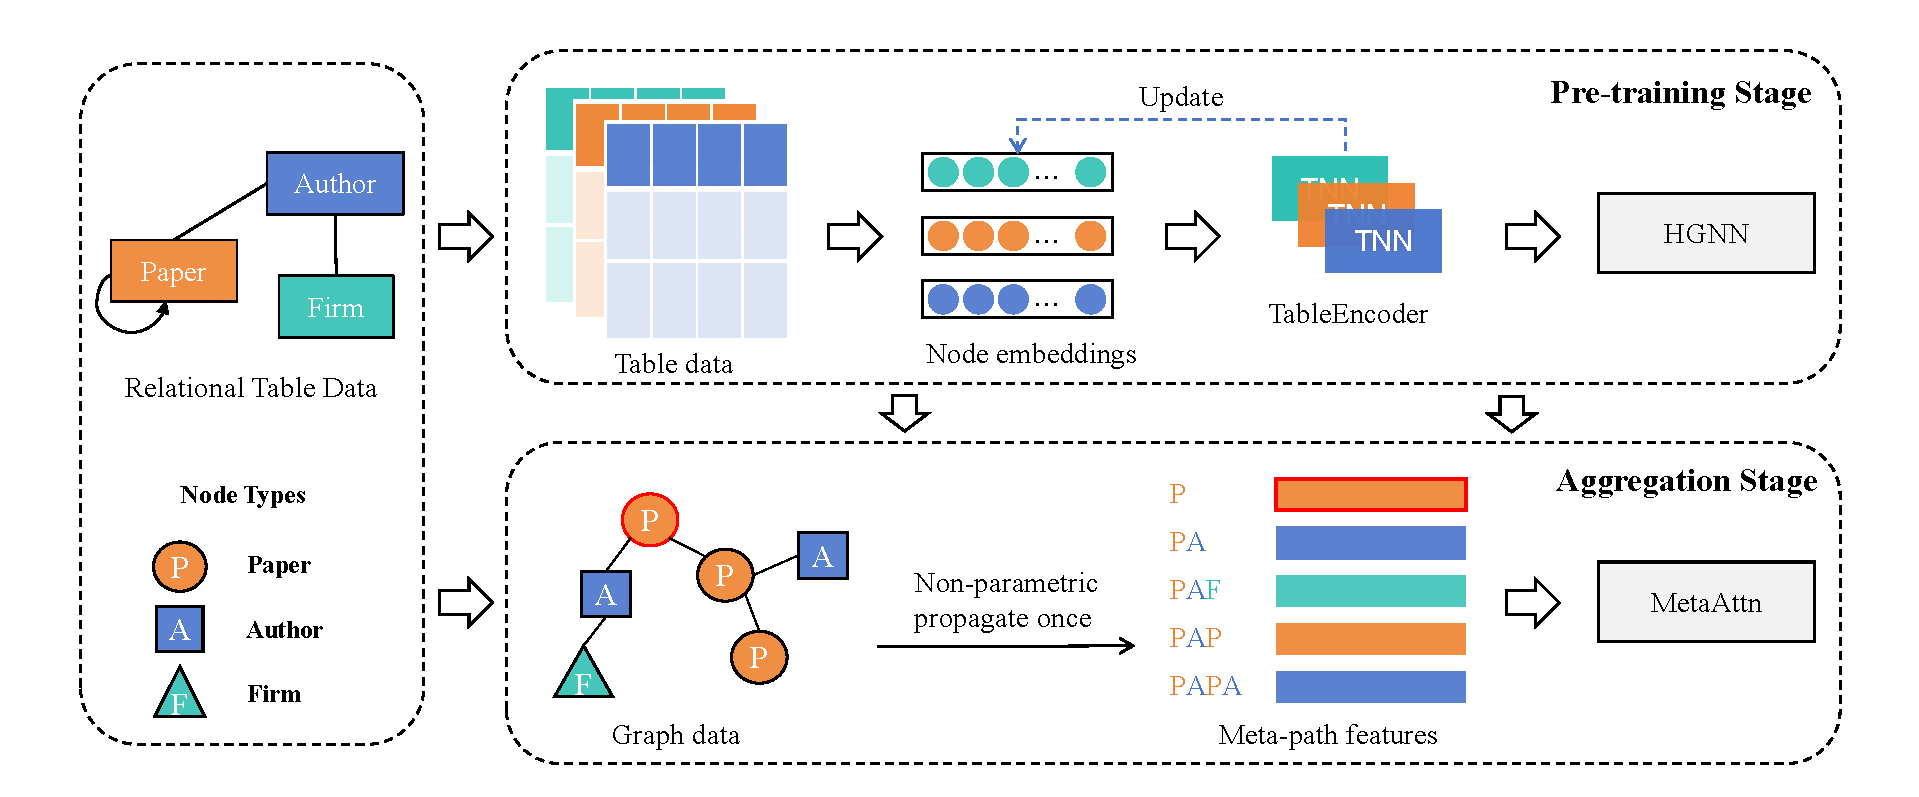
\includegraphics[width=\textwidth]{figures/metartl/fig1.pdf}
  \caption{MetaRTL 的两阶段总体结构}
  \label{fig:metartl-overview}
\end{figure}

% !TEX root = ../main.tex

\section{初始节点表示学习}
\label{sec:metartl-pretrain}

设 $\mathcal V_\tau$ 为类型 $\tau\in\mathcal T_v$ 的节点集合，
$D_\tau$ 为对应表格的原始行。MetaRTL 对不同类型分别设置表格神经网络
$f_\tau$，将异构字段编码到共同的 $d$ 维空间。对一个采样批次 $i$，
其类型为 $\tau$ 的节点索引集合记作 $\mathcal B_{\tau}^{(i)}$，初始表示为
\begin{equation}
  X_{\tau}^{(i)}
  = f_\tau\!\left(D_\tau[\mathcal B_{\tau}^{(i)}]\right)
  \in \mathbb R^{|\mathcal B_{\tau}^{(i)}|\times d}.
  \label{eq:metartl-tnn}
\end{equation}
表格编码器处理行内字段，异构图网络处理行间关系，两者承担不同的建模职责。
该设计与基于表格编码器和异构 GraphSAGE 的关系深度学习基线具有可比性
\cite{fey2024rdl,hamilton2017graphsage}。

第一阶段从训练种子出发采样小批次子图
$\mathcal G_i=(\mathcal V_i,\mathcal E_i)$，并用两层异构图网络聚合不同关系
类型的邻域信息。若 $g_{\omega}$ 表示异构图网络，$q_{\psi}$ 为任务预测头，
则预训练目标可写为
\begin{equation}
  \min_{\theta,\omega,\psi}
  \sum_{i\in\mathcal I_{\mathrm{train}}}
  \mathcal L_{\mathrm{task}}\!\left(
    q_\psi\!\left(g_\omega(
      \{f_{\tau,\theta}(D_\tau[\mathcal B_\tau^{(i)}])\}_{\tau},
      \mathcal G_i)\right),\,Y_i
  \right),
  \label{eq:metartl-pretrain}
\end{equation}
其中 $\mathcal L_{\mathrm{task}}$ 表示与预测任务对应的损失函数。
实验中预训练阶段进行五个训练轮次，其目的在于得到可供路径传播的节点
初始表示，而非将浅层图网络的输出直接作为最终结果。
预训练结束后，使用训练得到的表格编码器为后续阶段涉及的节点生成
$X_\tau\in\mathbb R^{|\mathcal V_\tau|\times d}$，并在第二阶段固定这些初始表示。

\section{基于元路径的非参数特征传播}
\label{sec:metartl-metapath}

元路径是定义在关系模式上的类型序列
\begin{equation}
  \mathcal P:\quad
  \tau_s=\tau_0\longrightarrow\tau_1\longrightarrow\cdots
  \longrightarrow\tau_\ell=\tau_t,
  \label{eq:metartl-path}
\end{equation}
其中 $\tau_s$ 和 $\tau_t$ 分别为源类型和预测目标类型。不同的类型序列
对应不同的跨表语义，例如“论文—作者—机构”与“论文—作者—论文”
即使有共同的起点，也描述不同的关联\cite{dong2017metapath2vec}。
令 $A_{\tau_j\leftarrow\tau_{j-1}}$ 为沿相应关系从
$\tau_{j-1}$ 聚合到 $\tau_j$ 的度归一化矩阵，则路径 $\mathcal P$ 的
传播矩阵为
\begin{equation}
  A^{\mathcal P}
  =A_{\tau_t\leftarrow\tau_{\ell-1}}\cdots
   A_{\tau_2\leftarrow\tau_1}
   A_{\tau_1\leftarrow\tau_s}.
  \label{eq:metartl-path-adj}
\end{equation}
这一乘积描述沿指定关系序列的特征传递，不含需要反向传播更新的参数。
在数据准备阶段复用较短路径的中间结果，得到候选元路径的传播矩阵，
再在训练批次中按目标节点和可用源节点索引截取。设
$\mathcal B_t$ 为批次目标节点，$\mathcal B_s$ 为该路径涉及的源节点，
则对应的批次特征为
\begin{equation}
  H_{\mathcal P}^{(\mathcal B)}
  =A^{\mathcal P}[\mathcal B_t,\mathcal B_s]\,
   X_{\tau_s}[\mathcal B_s,:]
  \in\mathbb R^{|\mathcal B_t|\times d}.
  \label{eq:metartl-path-feature}
\end{equation}
若 $\mathcal B_s$ 未覆盖路径矩阵中所有非零源节点，该式表示相应批次范围内的
路径特征；批次采样范围因此也是实验配置的一部分。将零跳路径定义为
$H_0=X_{\tau_t}[\mathcal B_t,:]$，可同时保留目标表自身字段信息。

与在每轮训练中反复执行深层可训练邻域传播相比，路径矩阵可跨训练轮次复用。
不过，矩阵乘积可能产生比原始边集更稠密的中间结果，因此这种预计算并非
无条件地节省时间或内存；其实际成本取决于关系模式、最大跳数、非零元数量
和存储策略。

\section{MetaAttn 路径语义融合}
\label{sec:metartl-attn}

MetaAttn 由元路径自注意力和全局节点交叉注意力两条分支组成，如
图~\ref{fig:metartl-metaattn} 所示。前者选择不同连接路径承载的信息，
后者使批次中的目标节点访问跨批共享的原型表示。

\begin{figure}[htbp]
  \centering
  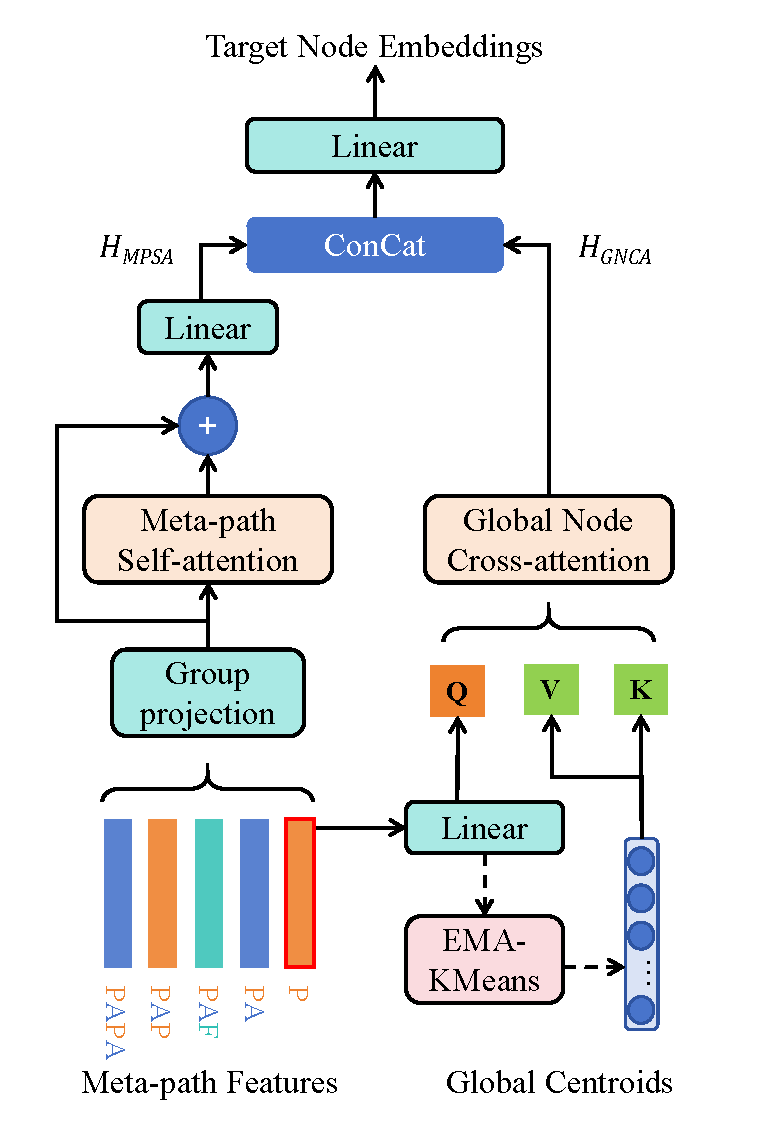
\includegraphics[width=0.50\textwidth]{figures/metartl/fig22.pdf}
  \caption{MetaAttn 的路径自注意力与共享原型交叉注意力结构}
  \label{fig:metartl-metaattn}
\end{figure}

\subsection{元路径自注意力}

令 $\Phi$ 为候选元路径集合，$m=|\Phi|$。对每一条路径的特征
$H_{\mathcal P}^{(\mathcal B)}$，按照其源节点类型 $\tau_s(\mathcal P)$
应用类型特定线性映射，并沿路径维堆叠，得到
\begin{equation}
  Z_{\mathcal B}
  =\operatorname{Stack}_{\mathcal P\in\Phi}
  \!\left(
    H_{\mathcal P}^{(\mathcal B)}
    W_{\tau_s(\mathcal P)}+b_{\tau_s(\mathcal P)}
  \right)
  \in\mathbb R^{|\mathcal B_t|\times m\times d}.
  \label{eq:metartl-stack}
\end{equation}
这样，同一源表类型可共享线性映射，而每条路径仍保留独立的位置。
对于每个目标节点，以其 $m$ 条路径特征为注意力序列，执行
\begin{equation}
  \operatorname{Attn}(Q,K,V)
  =\operatorname{softmax}\!\left(\frac{QK^\top}{\sqrt d}\right)V.
  \label{eq:metartl-attn}
\end{equation}
自注意力为不同路径建立依赖关系\cite{vaswani2017attention}。
将结果与输入作残差相加，再经过路径维聚合及线性投影，得到
\begin{equation}
  H_{\mathrm{MPSA}}
  =\operatorname{Proj}_{\Phi\rightarrow d}
  \!\left(\operatorname{SelfAttn}(Z_{\mathcal B})+Z_{\mathcal B}\right)
  \in\mathbb R^{|\mathcal B_t|\times d}.
  \label{eq:metartl-mpsa}
\end{equation}
其中 $\operatorname{Proj}_{\Phi\rightarrow d}$ 为作用于路径维的
可训练投影，将每个目标节点的多条路径表示映射为一个 $d$ 维向量。

\subsection{全局节点交叉注意力与输出}

仅从采样批次取得路径特征可能遗漏批次外的语义。MetaAttn 因此维护
$c$ 个跨批共享的原型向量
$C\in\mathbb R^{c\times d}$，以零跳目标节点特征作为查询，
以原型作为键和值，计算
\begin{equation}
  H_{\mathrm{GNCA}}
  =\operatorname{CrossAttn}(H_0W_Q,\;C,\;C).
  \label{eq:metartl-gnca}
\end{equation}
训练过程中采用基于 K-Means 的指数滑动平均规则，根据目标节点特征
更新 $C$。原型在批次之间共享，使目标节点能够利用批次外的统计信息，
同时避免与全图所有节点逐一计算注意力。
这一分支与使用共享全局节点的图注意力设计有关\cite{kong2023goat}。

两条分支的输出拼接后，由线性层生成最终目标节点表示：
\begin{equation}
  H_{\mathrm{out}}
  =W_F[H_{\mathrm{MPSA}}\Vert H_{\mathrm{GNCA}}]+b_F,
  \qquad
  \widehat Y=q(H_{\mathrm{out}}).
  \label{eq:metartl-output}
\end{equation}
第二阶段固定初始节点表示，并通过任务损失函数优化类型映射、
注意力模块与预测头的参数。预测头根据分类或回归任务设置，
分别输出类别预测值或连续数值。

\section{计算特征与方法边界}
\label{sec:metartl-complexity}

从消息传递的角度，可以把式~\eqref{eq:metartl-path-adj} 展开为
\begin{equation}
  H_{\mathcal P}^{(0)}=X_{\tau_s},\qquad
  H_{\mathcal P}^{(j)}
  =A_{\tau_j\leftarrow\tau_{j-1}}H_{\mathcal P}^{(j-1)},
  \quad j=1,\ldots,\ell.
  \label{eq:metartl-recursion}
\end{equation}
由矩阵乘法的结合律，
$H_{\mathcal P}^{(\ell)}=A^{\mathcal P}X_{\tau_s}$。
因此，长度为 $\ell$ 的元路径传播可解释为 $\ell$ 步沿指定关系类型
的无参数消息聚合，MetaAttn 则对多个路径的结果进行可训练融合。
全局节点交叉注意力使用共享原型而非数据库边，属于补充的
跨批信息通道，不能简单等同于同一图上的邻接消息传递。

设一个训练轮次中处理的目标节点总数为 $n_t$，路径数为 $m$，原型数为 $c$。
在隐藏维度为 $d$ 且常规稠密注意力实现下，路径自注意力及类型映射的
计算量约为
$\mathcal O\!\left(n_t(m^2d+md^2)\right)$；
目标节点到 $c$ 个原型的注意力另需约
$\mathcal O(n_tcd)$ 的相似度与加权计算。
预训练阶段的代价由表格编码器的字段处理以及采样边上的两层消息传递构成，
不能只用图边数表征。

离线路径矩阵的计算量和内存量还取决于
$\sum_{\mathcal P\in\Phi}\operatorname{nnz}(A^{\mathcal P})$
及中间稀疏矩阵乘积的非零元增长。因而，只有在路径集合和关系稀疏度
得到控制时，才能期待该阶段保持较好的可扩展性。本章后面的时间曲线
检验了固定平均出度的合成图设置；它不等同于所有关系数据库上的
复杂度保证。

% !TEX root = ../main.tex

\section{实验设置}
\label{sec:metartl-setup}

\subsection{数据集、任务与评价指标}

实验采用 SJTUTables 和 RelBench 两组公开关系表格数据
\cite{li2024rllm,robinson2024relbench}。
SJTUTables 包含 TACM12k、TLF2K 和 TML1M 三个多分类任务，
采用准确率评价；RelBench 包含七个数据库上的十二个
二分类任务和九个回归任务，分别采用 ROC-AUC 和平均绝对误差（MAE）
评价。两组数据共包含十个数据库、二十四项任务。
表~\ref{tab:metartl-datasets} 列出数据集规模和各数据集的关系跳数统计值；
候选元路径长度上限统一设置为四跳。

\begin{table}[htbp]
  \centering
  \caption{实验数据集规模}
  \label{tab:metartl-datasets}
  \begin{tabular}{lrrrr}
    \toprule
    数据集 & 表数 & 总行数 & 列数 & 统计表最大跳数 \\
    \midrule
    TACM12k    & 4  & 97,774     & 12  & 2 \\
    TLF2K      & 3  & 101,773    & 15  & 1 \\
    TML1M      & 3  & 1,010,132  & 20  & 2 \\
    rel-f1     & 9  & 97,606     & 77  & 3 \\
    rel-trial  & 15 & 5,852,157  & 140 & 3 \\
    rel-avito  & 8  & 20,679,117 & 43  & 2 \\
    rel-amazon & 3  & 24,291,489 & 15  & 2 \\
    rel-hm     & 3  & 33,265,846 & 37  & 2 \\
    rel-stack  & 7  & 38,109,828 & 51  & 3 \\
    rel-event  & 5  & 41,328,337 & 128 & 2 \\
    \bottomrule
  \end{tabular}
\end{table}

\subsection{对照方法与实现设置}

单表对照包括梯度提升树 LightGBM\cite{ke2017lightgbm}，以及
FTTransformer\cite{gorishniy2021tabular}、
Trompt\cite{chen2023trompt} 和
ExcelFormer\cite{chen2024excelformer} 三种表格深度学习模型。
多表对照包括 RelBench 中的 RDL、BRIDGE、RelGNN 和 LightRDL；
它们分别代表基于表格编码器和异构 GraphSAGE 的方法、使用受限辅助表
的图方法、复合关系消息传递方法以及利用预训练表格模型的方法
\cite{fey2024rdl,li2024rllm,chen2025relgnn,lachi2025lightrdl}。
单表方法通过连接目标表与对应特征表构造输入。
在包含多个辅助实体表的任务中，BRIDGE 使用与目标表最相关的一个辅助表。
RelGNN 与 LightRDL 根据其发布代码和论文描述复现；
对于缺少时间字段的 SJTUTables 数据，LightRDL 使用生成的时间戳。
这些设置构成相应方法在本实验中的实现条件。

MetaRTL 的预训练阶段进行五个训练轮次。模型采用四层、隐藏维度为
128 的表格编码器，两层、隐藏维度均为 128 的异构图网络，
候选元路径最长四跳，跨批共享原型数为 4096。表格编码器采用
ResNet 风格模块，异构图网络采用 GraphSAGE 风格模块。
RelBench 任务采用时间感知的均匀邻域采样，并遵循基准数据集的
任务划分及评价协议。

\section{预测性能比较}
\label{sec:metartl-results}

\subsection{SJTUTables 多分类任务}

表~\ref{tab:metartl-sjtu} 给出三个 SJTUTables 任务的准确率。
MetaRTL 在三项任务中均为表内最高：TACM12k 为 $46.54\%$，
TLF2K 为 $43.17\%$，TML1M 为 $37.09\%$。
其中 TACM12k 相对表内最佳单表方法 LightGBM 高
$10.84$ 个百分点；TLF2K 和 TML1M 相对各自最强的
其他多表方法 BRIDGE 分别高 $0.97$ 和 $0.89$ 个百分点。
三项任务的提升幅度存在差异，表明模型收益与数据集特征及任务有关。

\begin{table}[htbp]
  \centering
  \caption{SJTUTables 多分类任务的准确率（\%，越高越好）}
  \label{tab:metartl-sjtu}
  \begin{tabular}{lrrr}
    \toprule
    方法 & TACM12k & TLF2K & TML1M \\
    \midrule
    LightGBM     & 35.70 & 35.52 & 26.66 \\
    FTTransformer & 14.88 & 15.80 & 28.62 \\
    Trompt       & 12.42 & 13.41 & 27.85 \\
    ExcelFormer  & 17.13 & 20.61 & 31.90 \\
    RDL          & 19.23 & 19.58 & 26.93 \\
    RelGNN       & 18.19 & 20.31 & 27.12 \\
    BRIDGE       & 25.60 & 42.20 & 36.20 \\
    LightRDL     & 24.94 & 39.17 & 35.77 \\
    \textbf{MetaRTL} & \textbf{46.54} & \textbf{43.17} & \textbf{37.09} \\
    \bottomrule
  \end{tabular}
\end{table}

\subsection{RelBench 分类与回归任务}

表~\ref{tab:metartl-relbench-cls} 和表~\ref{tab:metartl-relbench-reg}
给出二十一项 RelBench 任务的预测结果。
为节约版面，表头中 FT、Excel、RGNN、BR 和 L-RDL
分别表示 FTTransformer、ExcelFormer、RelGNN、BRIDGE 和 LightRDL。
MetaRTL 在十二个分类任务中的九个取得单独最高 ROC-AUC，
在 \texttt{user-badge} 上与 RelGNN 并列最高；在九个回归任务中的
八个取得最低 MAE。综合来看，二十一项任务中有十七项单独最优、
一项并列最优，另有三项未达到最优。分类和回归任务的平均名次
分别为 $1.33$ 和 $1.67$。

\begin{table}[p]
  \centering
  \caption{RelBench 二分类任务的 ROC-AUC（越高越好）}
  \label{tab:metartl-relbench-cls}
  \resizebox{\textwidth}{!}{%
  \begin{tabular}{llrrrrrrrrr}
    \toprule
    数据集 & 任务 & LightGBM & FT & Trompt & Excel & RDL & RGNN & BR & L-RDL & MetaRTL \\
    \midrule
    rel-f1 & driver-top3       & .7392 & .7362 & .7317 & .7522 & .7723 & .8086 & .7713 & .7916 & .8415 \\
           & driver-dnf        & .6856 & .6831 & .6752 & .6720 & .7125 & .6706 & .7016 & .6863 & .7418 \\
    rel-trial & study-outcome   & .7009 & .6239 & .6573 & .6731 & .6902 & .6916 & .6898 & .6815 & .7013 \\
    rel-avito & user-clicks     & .5360 & .5132 & .5423 & .5532 & .6576 & .6613 & .5501 & .6411 & .6614 \\
              & user-visits    & .5305 & .5210 & .5611 & .5501 & .6599 & .6547 & .5616 & .6239 & .6587 \\
    rel-amazon & user-churn     & .5222 & .5230 & .5310 & .5209 & .7042 & .6544 & .5351 & .6917 & .7101 \\
               & item-churn    & .6254 & .6415 & .5982 & .6250 & .8281 & .8264 & .6993 & .8120 & .8290 \\
    rel-hm & user-churn        & .5521 & .5013 & .5419 & .5395 & .7011 & .6810 & .5933 & .6713 & .6795 \\
    rel-stack & user-engagement & .6339 & .6002 & .6573 & .6920 & .9047 & .8995 & .7974 & .8902 & .9120 \\
              & user-badge     & .6343 & .6036 & .6282 & .6713 & .8886 & .8898 & .8790 & .8671 & .8898 \\
    rel-event & user-repeat    & .6804 & .6910 & .6717 & .6973 & .7560 & .7307 & .7530 & .7132 & .7604 \\
              & user-ignore    & .7993 & .7569 & .7731 & .7792 & .7514 & .7911 & .7616 & .7630 & .8703 \\
    \midrule
    \multicolumn{2}{l}{平均名次} & 6.25 & 8.00 & 7.33 & 6.83 & 2.92 & 3.33 & 4.83 & 4.17 & 1.33 \\
    \bottomrule
  \end{tabular}}
\end{table}

\begin{table}[p]
  \centering
  \caption{RelBench 回归任务的 MAE（越低越好）}
  \label{tab:metartl-relbench-reg}
  \resizebox{\textwidth}{!}{%
  \begin{tabular}{llrrrrrrrrr}
    \toprule
    数据集 & 任务 & LightGBM & FT & Trompt & Excel & RDL & RGNN & BR & L-RDL & MetaRTL \\
    \midrule
    rel-f1 & driver-position & 4.170 & 4.210 & 4.191 & 4.112 & 4.172 & 4.250 & 4.179 & 4.170 & 3.987 \\
    rel-trial & study-adverse & 44.011 & 44.490 & 45.397 & 45.552 & 44.473 & 44.461 & 44.773 & 43.910 & 43.102 \\
              & site-success & .425 & .431 & .440 & .429 & .400 & .355 & .431 & .411 & .350 \\
    rel-avito & ad-ctr        & .041 & .049 & .045 & .050 & .041 & .039 & .044 & .040 & .040 \\
    rel-amazon & user-ltv     & 16.783 & 16.930 & 16.606 & 17.001 & 14.313 & 16.783 & 15.374 & 14.310 & 14.102 \\
               & item-ltv    & 60.569 & 60.319 & 61.424 & 59.983 & 50.053 & 48.826 & 60.441 & 48.112 & 46.176 \\
    rel-hm & item-sales      & .076 & .092 & .073 & .073 & .056 & .054 & .071 & .044 & .039 \\
    rel-stack & post-votes    & .068 & .074 & .080 & .070 & .065 & .065 & .066 & .064 & .060 \\
    rel-event & user-attendance & .264 & .270 & .281 & .264 & .258 & .248 & .259 & .260 & .241 \\
    \midrule
    \multicolumn{2}{l}{平均名次} & 5.72 & 7.72 & 7.72 & 6.78 & 3.89 & 3.78 & 5.50 & 2.61 & 1.67 \\
    \bottomrule
  \end{tabular}}
\end{table}

分类结果中，\texttt{rel-f1} 的 \texttt{driver-top3} 与
\texttt{driver-dnf} 分别达到 $0.8415$ 和 $0.7418$；
\texttt{rel-event} 的 \texttt{user-ignore} 达到 $0.8703$。
但 rel-avito 的 user-visits 任务和 rel-hm 的 user-churn 任务
分别略低于最优的 RDL 结果。回归结果中，
rel-amazon 的 item-ltv 任务的 MAE 为 $46.176$，
低于表中其他方法；rel-avito 的 ad-ctr 任务的 $0.040$
则高于 RelGNN 的 $0.039$。这些反例说明不同数据库和任务对
长路径信息及注意力融合的需求并不一致。

\section{消融实验与两阶段作用}
\label{sec:metartl-ablation}

在 \texttt{rel-f1} 数据集的三个任务上，分别去掉表格编码器预训练、
元路径特征和全局节点交叉注意力，结果见表~\ref{tab:metartl-ablation}。
不使用元路径特征时，\texttt{driver-top3} 的 ROC-AUC
由 $0.8415$ 降至 $0.6294$，\texttt{driver-position} 的
MAE 从 $3.987$ 升至 $4.870$，说明路径语义是该组任务中的
关键输入。去掉预训练同样导致三项指标下降。
去掉全局交叉注意力的影响相对较小，但三个任务均出现退化。
上述结果说明，在这三个任务中，元路径特征对预测性能的影响最为明显。

\begin{table}[htbp]
  \centering
  \caption{MetaRTL 在 rel-f1 数据集上的模块消融}
  \label{tab:metartl-ablation}
  \begin{tabular}{lrrr}
    \toprule
    方法 & driver-top3 $\uparrow$ & driver-dnf $\uparrow$ & driver-position $\downarrow$ \\
    \midrule
    去掉表格编码器预训练 & .7311 & .6761 & 4.319 \\
    去掉元路径特征       & .6294 & .6013 & 4.870 \\
    去掉全局节点交叉注意力 & .8389 & .7216 & 4.110 \\
    完整 MetaRTL         & .8415 & .7418 & 3.987 \\
    \bottomrule
  \end{tabular}
\end{table}

图~\ref{fig:metartl-stage} 进一步比较预训练阶段和完整聚合阶段的
预测结果。在图示的三个 F1 数据集任务上，第二阶段的
ROC-AUC 更高、MAE 更低。该观察与两阶段分工一致：
第一阶段形成可用的初始表示，第二阶段再引入路径和原型信息。
两阶段的性能差异反映了路径特征与注意力聚合共同引入后的效果，
各模块的作用进一步由表~\ref{tab:metartl-ablation} 中的消融实验体现。

\begin{figure}[htbp]
  \centering
  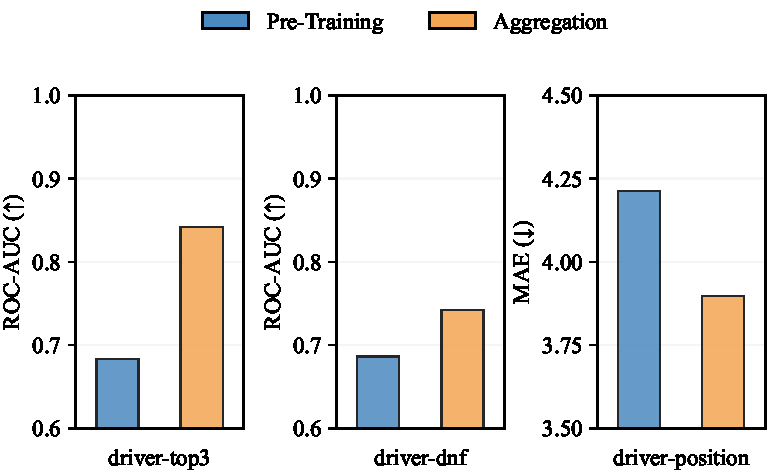
\includegraphics[width=0.88\textwidth]{figures/metartl/12cmp_subplots.pdf}
  \caption{MetaRTL 预训练阶段与聚合阶段的预测表现}
  \label{fig:metartl-stage}
\end{figure}

\section{预训练轮次与规模分析}
\label{sec:metartl-efficiency}

图~\ref{fig:metartl-epochs} 比较不同预训练轮次。
在 \texttt{rel-f1} 的三个任务上，单个 epoch 通常不足以得到较好的
初始表示；五个 epoch 相比一个 epoch 明显改善。
此后曲线并非一致单调：\texttt{driver-top3} 在二十个 epoch
附近也有较高值，而 \texttt{driver-dnf} 与回归任务的最优位置
不同。因此，五轮预训练能够在较少迭代次数下获得较好的初始表示，
但不同任务对应的最优轮次仍存在差异。

\begin{figure}[htbp]
  \centering
  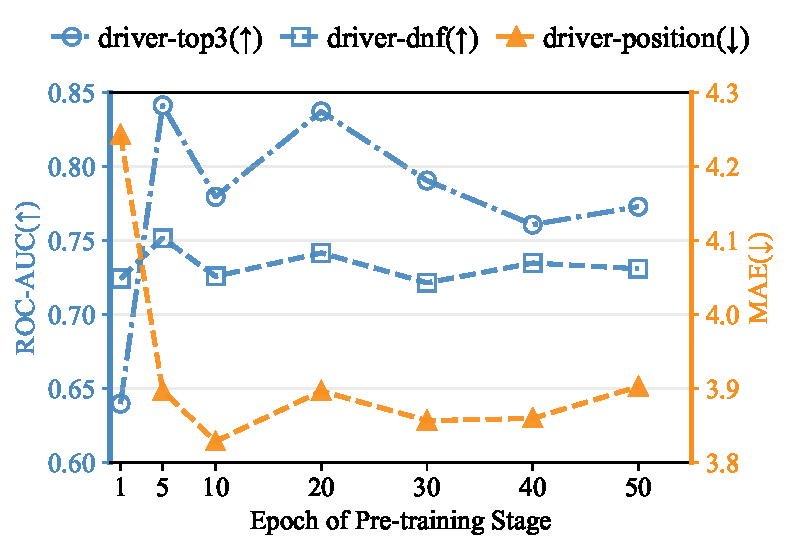
\includegraphics[width=0.78\textwidth]{figures/metartl/k.pdf}
  \caption{不同预训练轮次下的 MetaRTL 表现}
  \label{fig:metartl-epochs}
\end{figure}

为考察模型随图规模变化的运行时间，构造平均出度固定、
目标节点占总节点数 $1\%$ 的合成图，
观察节点数与训练时间的关系。图~\ref{fig:metartl-time}
显示，在该固定出度设置下，总时间随节点数增长大致呈线性趋势；
预训练和聚合两阶段均有不可忽略的时间开销。
在平均出度固定的条件下，该结果表明训练时间随节点规模近似线性增长。
关系模式与路径矩阵稀疏度发生变化时，离线传播矩阵的计算和存储开销
也会随之改变，因此还需结合具体数据库结构分析预计算成本。

\begin{figure}[htbp]
  \centering
  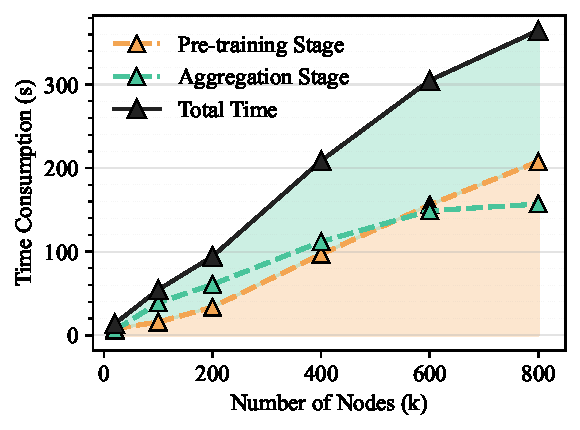
\includegraphics[width=0.78\textwidth]{figures/metartl/time.pdf}
  \caption{固定平均出度的合成图上节点数与训练时间的关系}
  \label{fig:metartl-time}
\end{figure}


\section{本章小结}

本章介绍了 MetaRTL 的两阶段设计。有限轮次的表格编码器与浅层异构图网络提供
初始表示；元路径传播将连接模式显式转化为候选特征；MetaAttn 再融合路径语义与
共享原型信息。在十个数据库、二十四项任务的实验中，MetaRTL 在三个
SJTUTables 任务上均取得最高准确率，在二十一项 RelBench 任务中取得十七项
单独最优和一项并列最优。消融实验表明，初始表示学习与元路径特征
对 \texttt{rel-f1} 数据集上的三项预测任务均有积极作用。元路径矩阵的
存储规模受路径数量及矩阵稀疏度影响，是方法应用于更大规模数据库时
需要考虑的因素。

MetaRTL 回答的是跨表信息怎样形成有效表示。后续章节讨论 RelX 怎样向训练过程
供给所需数据，两项工作的实验结果分别报告。

% !TEX root = ../main.tex

\chapter{大规模关系表格数据可扩展训练框架 RelX 的设计与实现}
\label{chap:relx-design}

\section{问题定义与设计目标}
\thesisplaceholder{界定大规模关系表格训练的输入、资源开销与可扩展性目标；分析数据规模增长时全量特征物化的内存开销，以及逐批准备对训练吞吐的影响。}

\section{RelX 总体架构}
\thesisplaceholder{绘制离线准备与在线训练的总体架构图，说明采样、特征准备和模型训练三个在线阶段的数据流及模块边界。}

\section{离线结构与统计准备}
\thesisplaceholder{说明模式、拓扑和必要统计量的准备过程，区分必须常驻的结构与按需获取的原始行及编码特征。}

\section{采样计划与按需特征读取}
\thesisplaceholder{定义采样计划的数据结构、节点请求去重和逆映射，说明如何从数据库读取所需行并恢复原批次的节点顺序。}

\section{异构字段编码与批次组装}
\thesisplaceholder{说明数值、类别、文本字段从原始行到模型输入的转换、组装进程的职责以及跨进程传递的对象。}

\section{分层缓存与特征复用}
\thesisplaceholder{描述原始行、已编码行、文本向量等缓存层的键、准入、失效和预算；说明不同负载下可能的收益与代价。}

\section{有界并行流水线}
\thesisplaceholder{说明采样、组装和训练的生产者—消费者关系、有界队列、在途窗口、执行顺序及异常处理，并区分批内依赖与跨批重叠。}

\section{语义一致性与适用范围}
\thesisplaceholder{列明任务划分、时间可见性、邻居采样、节点标识、字段类型和编码规则等不变性约束；说明当前拓扑驻内存等实现边界。}

\section{本章小结}
\thesisplaceholder{归纳 RelX 在数据规模增长条件下控制内存开销、减少重复准备和维持训练吞吐的设计，连接下一章的验证实验。}

% !TEX root = ../main.tex

\chapter{RelX 的实验评估与分析}
\label{chap:relx-evaluation}

\section{实验环境与对照设置}
\thesisplaceholder{记录数据库、任务、模型、机器、软件版本、批大小、轮数、种子和缓存预算；区分冷启动与热启动，并固定公平对照条件。}

\section{输入正确性与训练质量}
\thesisplaceholder{比较基线与 RelX 的采样计划、输入张量、时间约束、损失及预测指标，说明一致性检查的方法和误差容忍范围。}

\section{端到端耗时与训练吞吐}
\thesisplaceholder{报告初始化、在线训练、启动和排空的墙钟时间，以及实际完成批次的吞吐；分析模型等待数据的时间。}

\section{整作业内存与存储开销}
\thesisplaceholder{使用进程树 PSS 或隔离环境中的内存峰值，分别报告拓扑、组装进程、队列和缓存开销；补充磁盘占用。}

\section{数据规模扩展实验}
\thesisplaceholder{在可比的模型与训练配置下改变数据库规模，报告端到端耗时、训练吞吐、内存峰值与存储开销随规模变化的趋势，并分析主要瓶颈。}

\section{组件消融与参数敏感性}
\thesisplaceholder{在相同预算下考察组装进程数、请求去重、各层缓存、跨批复用窗口和在途队列；记录命中率及实际生效情况。}

\section{不同工作负载下的表现与局限}
\thesisplaceholder{按长文本、宽数值表、重复实体比例等负载特征解释加速或退化；区分历史观测、短程受控实验与最终配对结果。}

\section{本章小结}
\thesisplaceholder{基于最终实验数据总结 RelX 的输入正确性、训练效率、内存开销及规模扩展表现。}

% !TEX root = ../main.tex

\chapter{总结与展望}
\label{chap:conclusion}

\section{全文工作总结}
\thesisplaceholder{分别总结 MetaRTL 在跨表语义建模方面的工作与 RelX 在大规模关系表格数据可扩展训练方面的工作，概述各自有实验支持的结论。}

\section{研究局限}
\thesisplaceholder{说明 MetaRTL 与 RelX 尚未完成联合部署，以及数据规模、系统内存、实验覆盖与可复现性方面的实际边界。}

\section{未来工作}
\thesisplaceholder{讨论两项工作的可能集成、拓扑外存化、缓存策略改进以及更完整的跨任务和跨平台验证。}


\printbibliography[heading=bibintoc]

% 待补充实验配置或推导细节时，可在此加入附录。
% \appendix
% \input{contents/appendix}

\backmatter
% !TEX root = ../main.tex

\begin{acknowledgements}
  \thesisplaceholder{在定稿阶段根据实际情况撰写致谢。}
\end{acknowledgements}

% !TEX root = ../main.tex

\begin{achievements}
  \thesisplaceholder{根据学校要求和真实成果填写攻读学位期间的论文、专利、项目等；未确认的成果不列入。}
\end{achievements}

% !TEX root = ../main.tex

\begin{resume}
  \thesisplaceholder{根据学校要求填写真实的教育经历、研究经历和联系方式。}
\end{resume}


\end{document}
